
\chapter{2. Linear PDEs: a structured grid example}

We start with the Poisson problem because it is the right place to start.  Though it is a cliche in applied mathematics, in solving it we will learn how to use key parts of \PETSc: we will build a structured grid using a \PETSc \pDMDA, then assemble a \pMat in parallel based on this grid, and then solve in parallel using a \pKSP object.

\section{A Poisson problem on a square domain}

The \emph{Laplacian}
    $$\grad^2 u = \Div(\grad u) = \frac{\partial^2 u}{\partial x^2} + \frac{\partial^2 u}{\partial y^2}$$
of a function $u(x,y)$ almost always appears in a mathematical model because the quantity $u$ is conserved in some sense, and because of an assumption that the flux of $u$ is, up to a coefficient, the gradient $\grad u$ \citep{Ockendonetal2003}.  The divergence ``$\Div$'' factor of the Laplacian arises from a connection between a flux integral over a closed surface and an integral over the interior of that surface, namely the divergence (Gauss-Green) theorem \citep[Appendix C]{Evans}.

Let $\mathcal{S}$ be the open unit square $(0,1)\times(0,1)$ and denote its boundary by ``$\partial\mathcal{S}$;'' this set is simply the union of four (closed) line segments.  The following is our \emph{Poisson problem} for this Chapter;  see Figure \ref{fig:unitsquare}:
\begin{marginfigure}
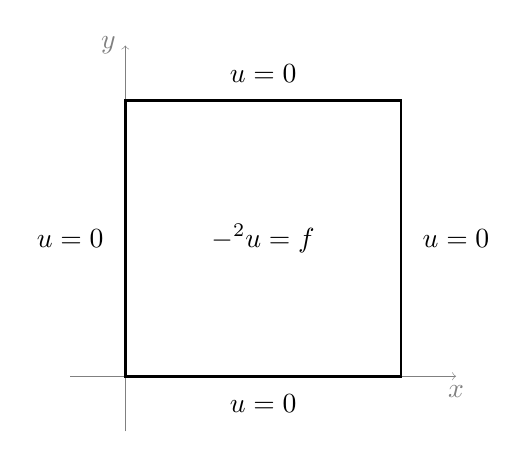
\begin{tikzpicture}[scale=3.5]
  \draw[->,gray,very thin] (-0.2,0.0) -- (1.2,0.0) node[below] {$x$};
  \draw[->,gray,very thin] (0.0,-0.2) -- (0.0,1.2) node[left] {$y$};
  \draw[line width=1.0pt] (0.0,0.0) -- (0.0,1.0) -- (1.0,1.0) -- (1.0,0.0) -- cycle;
  \node at (0.5,0.5) {$- \grad^2 u = f$};
  \node at (0.5,-0.1) {$u = 0$};
  \node at (0.5,1.1) {$u = 0$};
  \node at (-0.2,0.5) {$u = 0$};
  \node at (1.2,0.5) {$u = 0$};
\end{tikzpicture}
\caption{Our first, simple goal is to solve the Poisson equation on the unit square $\mathcal{S}$, with homogeneous Dirichlet boundary conditions.}
\label{fig:unitsquare}
\end{marginfigure}
\begin{align}
- \grad^2 u &= f \quad \text{ on } \mathcal{S}, \label{poissonsquare} \\
u &= 0 \quad \text{ on } \partial \mathcal{S}. \label{poissonsquarebcs}
\end{align}
The PDE \eqref{poissonsquare} is the \emph{Poisson equation} and equation \eqref{poissonsquarebcs} are \emph{homogeneous Dirichlet} boundary conditions.  Historically the problem \eqref{poissonsquare} and \eqref{poissonsquarebcs} is more properly called the \emph{Dirichlet problem}, but we call it ``Poisson'' because we will think about it flexibly with various boundary conditions (e.g.~in Chapter 3).  The problem must include boundary conditions, either Dirichlet ($u$ known) or Neumann (derivative of $u$ known), or a combination, it is to determine a unique solution.

The Poisson problem may model the electrostatic potential, the equilibrium distribution from certain random walks, the distribution of temperature in a conducting object at steady state, and many other other physical phenomena.  For example, in the context of heat conduction Fourier's law says $\bq = -k \grad u$, where $k$ is approximately constant if the variation in $u$ is not too large.  Conservation of energy for a solid says $c\rho \partial u/\partial t = - \Div\bq + f$ if $f$ describes a heat source within the domain.  At steady state these facts combine to give $0 = k \grad^2 u + f$, that is, Poisson's equation \eqref{poissonsquare}.  Holding the temperature fixed at zero along the boundary completes the problem.

For  the numerical approximation in this Chapter we will suppose that $f(x,y)$ is continuous (and bounded) on $\mathcal{S}$, so that we can compute its pointwise values.  With our homogeneous Dirichlet boundary conditions, and the assumptions on $f$, standard theory says that $u(x,y)$ exists and is continuous on the closed square $\overline{\mathcal{S}}$ \citep[Theorem 6 in section 5.6]{Evans}.\sidenote{A classical approach to showing existence starts by solving problem \eqref{poissonsquare} by Fourier series.  If $f$ is square-integrable then the coefficients $\hat f$ are square-integrable (Parseval's equality).  Because the Laplacian is elliptic and second-order, the coefficients $\hat u$ are square-integrable even when multiplied by the frequency squared.  By Cauchy-Schwarz, the Fourier series for $u$ is the limit of a sequence of continuous functions on $\overline{\mathcal{S}}$ which converge uniformly, so $u\in C^0(\overline{\mathcal{S}})$.}  Thus there is no ambiguity in the boundary condition ``$u=0$ on $\partial \mathcal{S}$,'' and also we can sensibly discuss the pointwise values $u(x,y)$.

Without any boundary conditions, the Poisson equation $-\grad^2 u = f$ alone is not a well-posed problem because if $u$ is a solution then $v=u+C$ is also a solution for any constant $C$.  (In fact there are constant solutions $w=C$ and many, many more to the Laplace equation $-\grad^2 w = 0$ on $\mathcal{S}$.)  However, with the Dirichlet boundary conditions in \eqref{poissonsquare}, the solution is unique if it exists \citep[Theorem 5 in section 2.2]{Evans}; \citep[subsection 5.2.1]{Ockendonetal2003}.


\section{Finite difference method: build the grid}

Because \eqref{poissonsquare} and \eqref{poissonsquarebcs} is a linear problem, finite-dimensional approximations of it are simply linear systems.  The approximation in this Chapter comes from applying a \emph{finite difference} (FD) method.  In Chapter 3 we will apply a finite element approach instead.

\begin{marginfigure}
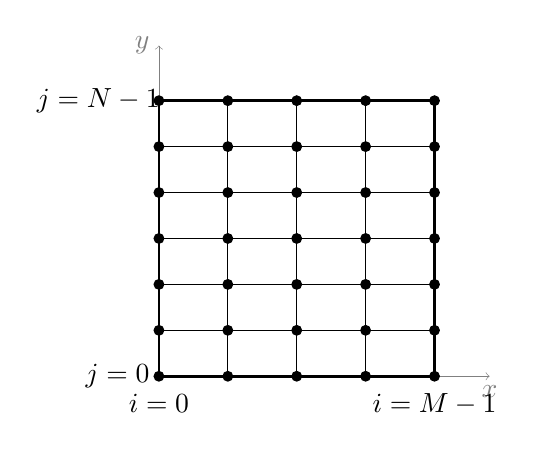
\begin{tikzpicture}[scale=3.5]
  \draw[->,gray,very thin] (0.0,0.0) -- (1.2,0.0) node[below] {$x$};
  \draw[->,gray,very thin] (0.0,0.0) -- (0.0,1.2) node[left] {$y$};
  \draw[line width=1.0pt] (0.0,0.0) -- (0.0,1.0) -- (1.0,1.0) -- (1.0,0.0) -- cycle;
  \node at (0.0,-0.1) {$i=0$};
  \node at (1.0,-0.1) {$i=M-1$};
  \node at (-0.15,0.0) {$j=0$};
  \node at (-0.22,1.0) {$j=N-1$};
  \pgfmathsetmacro\fourth{1.0/4.0}
  \pgfmathsetmacro\sixth{1.0/6.0}
  \draw[xstep=\fourth,ystep=\sixth,black,thin] (0.0,0.0) grid (1.0,1.0);
  \foreach \x in {0,...,4} {
    \foreach \y in {0,...,6} {
        \filldraw (\x * \fourth,\y * \sixth) circle (0.5pt);
    }
  }
\end{tikzpicture}
\caption{A grid on the unit square $\mathcal{S}$, with $M=5$ and $N=7$.}
\label{fig:unitsquaregrid}
\end{marginfigure}

To start our FD method we put a \emph{structured grid} of $MN$ points on the unit square, as in Figure \ref{fig:unitsquaregrid}, with spacing $h_x=1/(M-1)$ and $h_y=1/(N-1)$ in the two directions.  The grid coordinates are $x_i = i\, h_x$ for $i = 0,1,\dots,M-1$ and $y_j = j\, h_y$ and $j=0,1,\dots,N-1$.

The construction of such a two-dimensional (2D) grid, and the distribution of it across processors, will be our first new idea from \PETSc, beyond the basics in Chapter 1.  Consider the lines of code in Figure \ref{code:dmdacreatetwod}, which is an extract from \texttt{c2poisson.c}, which our Poisson problem and appears later in this Chapter.  These lines create a \PETSc \pDM object\sidenote{``\pDM'' might stand for ``data management'', but perhaps ``distributed mesh'' is better.} for a grid like Figure \ref{fig:unitsquaregrid}.

\clearpage
\cinputraw{dmdacreate2d.frag}{extract from c2poisson.c}{An example of creating a 2D \pDMDA.}{}{//START}{//STOP}{code:dmdacreatetwod}

A \pDM is an abstract type for describing the topology (connectedness) of a grid, \emph{and} the way it is distributed across \MPI processes, \emph{and} the way each process can access data from its neighbors.  The specific variable \texttt{da} in Figure \ref{code:dmdacreatetwod} has type ``\pDMDA'', which is the subclass of \pDM s which are structured grids.

\begin{marginfigure}
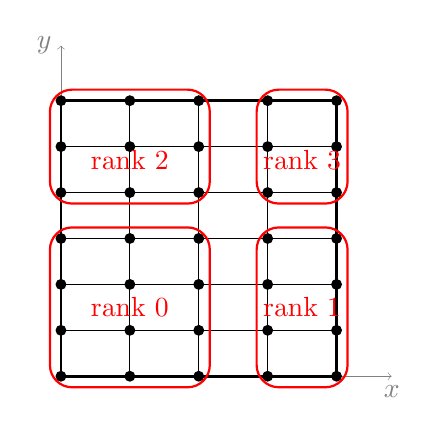
\begin{tikzpicture}[scale=3.5]
  \draw[->,gray,very thin] (0.0,0.0) -- (1.2,0.0) node[below] {$x$};
  \draw[->,gray,very thin] (0.0,0.0) -- (0.0,1.2) node[left] {$y$};
  \draw[line width=1.0pt] (0.0,0.0) -- (0.0,1.0) -- (1.0,1.0) -- (1.0,0.0) -- cycle;
  \pgfmathsetmacro\fourth{1.0/4.0}
  \pgfmathsetmacro\sixth{1.0/6.0}
  \draw[xstep=\fourth,ystep=\sixth,black,thin] (0.0,0.0) grid (1.0,1.0);
  \foreach \x in {0,...,4} {
    \foreach \y in {0,...,6} {
        \filldraw (\x * \fourth,\y * \sixth) circle (0.5pt);
    }
  }
  \pgfmathsetmacro\dd{0.04}
  \pgfmathsetmacro\od{1.04}
  \pgfmathsetmacro\xap{2*\fourth + 0.04}
  \pgfmathsetmacro\xbm{3*\fourth - 0.04}
  \pgfmathsetmacro\yap{3*\sixth + 0.04}
  \pgfmathsetmacro\ybm{4*\sixth - 0.04}
  \pgfmathsetmacro\xamid{1*\fourth}
  \pgfmathsetmacro\xbmid{3.5*\fourth}
  \pgfmathsetmacro\yamid{1.5*\sixth}
  \pgfmathsetmacro\ybmid{4.7*\sixth}
  \draw[thick,rounded corners=8pt,color=red]
    (-\dd,-\dd) -- (-\dd,\yap) -- (\xap,\yap) -- (\xap,-\dd) -- cycle;
  \node[color=red] at (\xamid,\yamid) {rank $0$};
  \draw[thick,rounded corners=8pt,color=red]
    (\xbm,-\dd) -- (\od,-\dd) -- (\od,\yap) -- (\xbm,\yap) -- cycle;
  \node[color=red] at (\xbmid,\yamid) {rank $1$};
  \draw[thick,rounded corners=8pt,color=red]
    (-\dd,\ybm) -- (\xap,\ybm) -- (\xap,\od) -- (-\dd,\od) -- cycle;
  \node[color=red] at (\xamid,\ybmid) {rank $2$};
  \draw[thick,rounded corners=8pt,color=red]
    (\xbm,\ybm) -- (\od,\ybm) -- (\od,\od) -- (\xbm,\od) -- cycle;
  \node[color=red] at (\xbmid,\ybmid) {rank $3$};
\end{tikzpicture}
\caption{The same grid as in Figure \ref{fig:unitsquaregrid}, distributed across four \MPI processes (i.e.~with \texttt{rank} $\in \{0,1,2,3\}$) automatically by \texttt{DMDACreate2d()}.}
\label{fig:unitsquaregridparallel}
\end{marginfigure}

If we do
\begin{Verbatim}[fontsize=\small]
  make c2poisson
  ./c2poisson -da_grid_x 5 -da_grid_y 7
\end{Verbatim}
then a structured grid will be created which is exactly as shown in Figure \ref{fig:unitsquaregrid}.  In this case all points of the grid are ``owned'' by the single process created when we run \texttt{c2poisson} (without \MPI).  However, if we run it with multiple \MPI processes by
\begin{Verbatim}[fontsize=\small]
  mpiexec -n N ./c2poisson -da_grid_x Mx -da_grid_y My
\end{Verbatim}
then \PETSc does the best it can to balance the load of \texttt{Mx}$\cdot$\texttt{My} grid points among \texttt{N} processes, with the restriction that each \MPI process owns a rectangular subgrid when we use a \pDMDA object to manage the grid.  For example, if we do
\begin{Verbatim}[fontsize=\small]
  mpiexec -n 4 ./c2poisson -da_grid_x 5 -da_grid_y 7
\end{Verbatim}
then the distributed structured grid shown in Figure \ref{fig:unitsquaregridparallel} will be created.  Neither \texttt{Mx}$=5$ nor \texttt{My}$=7$ is divisible by two, but \PETSc distributes the four ranks across the \texttt{Mx}$\cdot$\texttt{My}$=35$ nodes (grid points) relatively uniformly: the rank $0$ process owns 12 grid points and the rank $3$ process owns 6, while the other ranks are in between.  In this case the load is only balanced to within a factor of two, but larger grids will be better load-balanced.  

\begin{marginfigure}
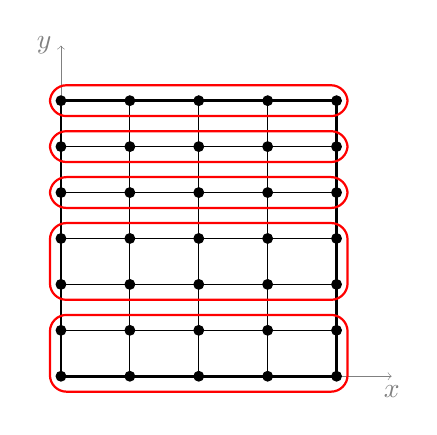
\begin{tikzpicture}[scale=3.5]
  \draw[->,gray,very thin] (0.0,0.0) -- (1.2,0.0) node[below] {$x$};
  \draw[->,gray,very thin] (0.0,0.0) -- (0.0,1.2) node[left] {$y$};
  \draw[line width=1.0pt] (0.0,0.0) -- (0.0,1.0) -- (1.0,1.0) -- (1.0,0.0) -- cycle;
  \pgfmathsetmacro\fourth{1.0/4.0}
  \pgfmathsetmacro\sixth{1.0/6.0}
  \draw[xstep=\fourth,ystep=\sixth,black,thin] (0.0,0.0) grid (1.0,1.0);
  \foreach \x in {0,...,4} {
    \foreach \y in {0,...,6} {
        \filldraw (\x * \fourth,\y * \sixth) circle (0.5pt);
    }
  }
  \pgfmathsetmacro\dd{0.04}
  \pgfmathsetmacro\od{1.04}
  \foreach \y in {0,2} {
    \pgfmathsetmacro\yup{\y * \sixth - 1.4 * \dd}  % less than 1.7 generates flaw?
    \pgfmathsetmacro\ydn{(\y + 1) * \sixth + 1.4 * \dd}
    \draw[thick,rounded corners=6pt,color=red]
      (-\dd,\ydn) -- (\od,\ydn) -- (\od,\yup) -- (-\dd,\yup) -- cycle;
  }
  \foreach \y in {4,5,6} {
    \pgfmathsetmacro\yup{\y * \sixth - 1.4 * \dd}  % less than 1.7 generates flaw?
    \pgfmathsetmacro\ydn{\y * \sixth + 1.4 * \dd}
    \draw[thick,rounded corners=6pt,color=red]
      (-\dd,\ydn) -- (\od,\ydn) -- (\od,\yup) -- (-\dd,\yup) -- cycle;
  }
\end{tikzpicture}
\caption{Processor domains are far from square if the total number of \MPI processes is prime, because only one dimension can be decomposed.  We show what \texttt{-dm\_view} reports for the same grid as in Figure \ref{fig:unitsquaregrid}, with \texttt{mpiexec -n 5}.}
\label{fig:unitsquaregridprime}
\end{marginfigure}

The observant reader may have already noted that the total number of processes \texttt{N}, in ``\texttt{mpiexec -n N},'' must not be prime if we are to get relatively-square processor domains in (portions of) the grid.  The ``bad'' result from running
\begin{Verbatim}[fontsize=\small]
  mpiexec -n 5 ./c2poisson -da_grid_x 5 -da_grid_y 7
\end{Verbatim}
is shown in Figure \ref{fig:unitsquaregridprime}.  Though the load may be acceptably balanced, each process' portion of the grid is not ``compact'' in the sense of having a small perimeter-to-area ratio.

The fifth and sixth arguments ``\texttt{-10}'' to \texttt{DMDACreate2d()} in Figure \ref{code:dmdacreatetwod} are used to set default dimensions $M=10$ and $N=10$, but we have seen how these defaults are overridden by runtime options \texttt{-da\_grid\_x} and \texttt{-da\_grid\_y}.  The command
 \begin{Verbatim}[fontsize=\small]
  mpiexec -n 4 ./c2poisson
\end{Verbatim}
distributes a $10\times 10$ grid aamong four processes as in Figure \ref{fig:unitsquaregrideight}, with each rank owning 25 nodes.  \PETSc can show the parallel layout by calling
\begin{Verbatim}[fontsize=\small]
  mpiexec -n 4 ./c2poisson -dm_view
\end{Verbatim}
or even
\begin{Verbatim}[fontsize=\small]
  mpiexec -n 4 ./c2poisson -dm_view draw -draw_pause 2
\end{Verbatim}
to see the grid graphically.

\begin{marginfigure}
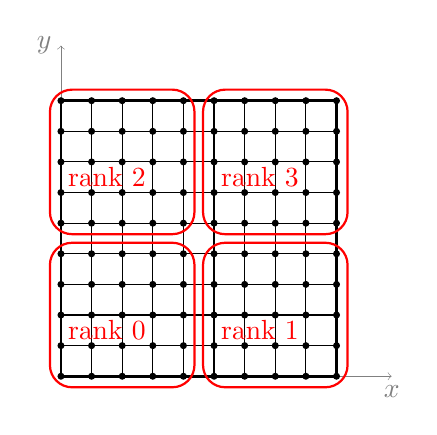
\begin{tikzpicture}[scale=3.5]
  \draw[->,gray,very thin] (0.0,0.0) -- (1.2,0.0) node[below] {$x$};
  \draw[->,gray,very thin] (0.0,0.0) -- (0.0,1.2) node[left] {$y$};
  \draw[line width=1.0pt] (0.0,0.0) -- (0.0,1.0) -- (1.0,1.0) -- (1.0,0.0) -- cycle;
  \pgfmathsetmacro\ninth{1.0/9.0}
  \draw[xstep=\ninth,ystep=\ninth,black,thin] (0.0,0.0) grid (1.0,1.0);
  \foreach \x in {0,...,9} {
    \foreach \y in {0,...,9} {
        \filldraw (\x * \ninth,\y * \ninth) circle (0.3pt);
    }
  }
  \pgfmathsetmacro\dd{0.04}
  \pgfmathsetmacro\od{1.04}
  \pgfmathsetmacro\ap{4*\ninth + 0.04}
  \pgfmathsetmacro\bm{5*\ninth - 0.04}
  \pgfmathsetmacro\amid{1.5*\ninth}
  \pgfmathsetmacro\bmid{6.5*\ninth}
  \draw[thick,rounded corners=8pt,color=red]
    (-\dd,-\dd) -- (-\dd,\ap) -- (\ap,\ap) -- (\ap,-\dd) -- cycle;
  \node[color=red] at (\amid,\amid) {rank $0$};
  \draw[thick,rounded corners=8pt,color=red]
    (\bm,-\dd) -- (\od,-\dd) -- (\od,\ap) -- (\bm,\ap) -- cycle;
  \node[color=red] at (\bmid,\amid) {rank $1$};
  \draw[thick,rounded corners=8pt,color=red]
    (-\dd,\bm) -- (\ap,\bm) -- (\ap,\od) -- (-\dd,\od) -- cycle;
  \node[color=red] at (\amid,\bmid) {rank $2$};
  \draw[thick,rounded corners=8pt,color=red]
    (\bm,\bm) -- (\od,\bm) -- (\od,\od) -- (\bm,\od) -- cycle;
  \node[color=red] at (\bmid,\bmid) {rank $3$};
\end{tikzpicture}
\caption{A well-balanced, compact-domain distribution of a $M=10$ by $N=10$ grid across four \MPI processes, created by \texttt{DMDACreate2d()}.}
\label{fig:unitsquaregrideight}
\end{marginfigure}

To explain the other options to \texttt{DMDACreate2d()} we start by quoting the \PETSc manual pages description:

\noindent\hrulefill
\begin{Verbatim}[fontsize=\small]
DMDACreate2d(MPI_Comm comm, DMBoundaryType bx, DMBoundaryType by,
  DMDAStencilType stype, PetscInt M, PetscInt N, PetscInt m, PetscInt n,
  PetscInt dof, PetscInt s, const PetscInt lx[], const PetscInt ly[],
  DM *da)
\end{Verbatim}
where
\small
\begin{itemize}[align=left]
\item[\texttt{comm}]   MPI communicator \\
\item[\texttt{bx,by}]  type of ghost nodes the array have; use one of \texttt{DM\_BOUNDARY\_NONE, DM\_BOUNDARY\_GHOSTED, DM\_BOUNDARY\_PERIODIC} \\
\item[\texttt{stype}] stencil type; use either \texttt{DMDA\_STENCIL\_BOX} or \texttt{DMDA\_STENCIL\_STAR} \\
\item[\texttt{M,N}]	   global dimension in each direction of the array; use \texttt{-M} and or \texttt{-N} to indicate that it may be set to a different value from the command line with \texttt{-da\_grid\_x <M> -da\_grid\_y <N>} \\
\item[\texttt{m,n}]   corresponding number of processors in each dimension (or \texttt{PETSC\_DECIDE} to have calculated) \\
\item[\texttt{dof}]     number of degrees of freedom per node \\
\item[\texttt{s}]       stencil width \\
\item[\texttt{lx,ly}]  arrays containing the number of nodes in each cell along the x and y coordinates, or \texttt{NULL}; if non-null, these must be of length as m and n, and the corresponding m and n cannot be \texttt{PETSC\_DECIDE}; the sum of the \texttt{lx[]} entries must be M, and the sum of the \texttt{ly[]} entries must be N \\
\item[\texttt{da}]      output: the resulting distributed array object 
\end{itemize}
\normalsize
\noindent\hrulefill
\medskip

\noindent In Figure \ref{code:dmdacreatetwod}, the first argument to \texttt{DMDACreate2d()} is the default parallel \MPI communicator including all \texttt{N} processes in ``\texttt{mpiexec -n N}.''  In the second and third arguments we have used ``\texttt{DM\_BOUNDARY\_NONE}'' because our Dirichlet boundary condition does not require communication to the next process' domain, nor periodic wrapping.  In the fourth argument we use \texttt{DMDA\_STENCIL\_STAR} because only cardinal neighbors of a grid point are used when forming the matrix; we will address the FD ``stencil'' below.  As already noted, the fifth and sixth arguments set $M=10,N=10$ as override-able grid defaults.  In the next two arguments, ``\texttt{PETSC\_DECIDE}'' tells \PETSc to decompose our grid over \MPI processes according to the size of (number of processes in) the \MPI communicator, and using \PETSc internal logic as illustrated above.  The next two arguments, in the ninth and tenth positions, say that our PDE is scalar (\texttt{dof}$=1$) and that the FD method only needs one neighbor in each \texttt{STENCIL\_STAR} direction (\texttt{s}$=1$).  The next two arguments are \texttt{NULL} because we are \emph{not} telling \PETSc any details about how to distribute processes over the grid; it \texttt{DECIDE}s for itself.  Finally, the \pDMDA object is created as an output.

The call to \texttt{DMDASetUniformCoordinates()} in Figure \ref{code:dmdacreatetwod} sets the domain to be $[0,1]\times[0,1]$.  The last two arguments are ignored in this case; they would set limits on the third dimension if \texttt{da} was created with \texttt{DMDACreate3d()}.

\begin{figure}
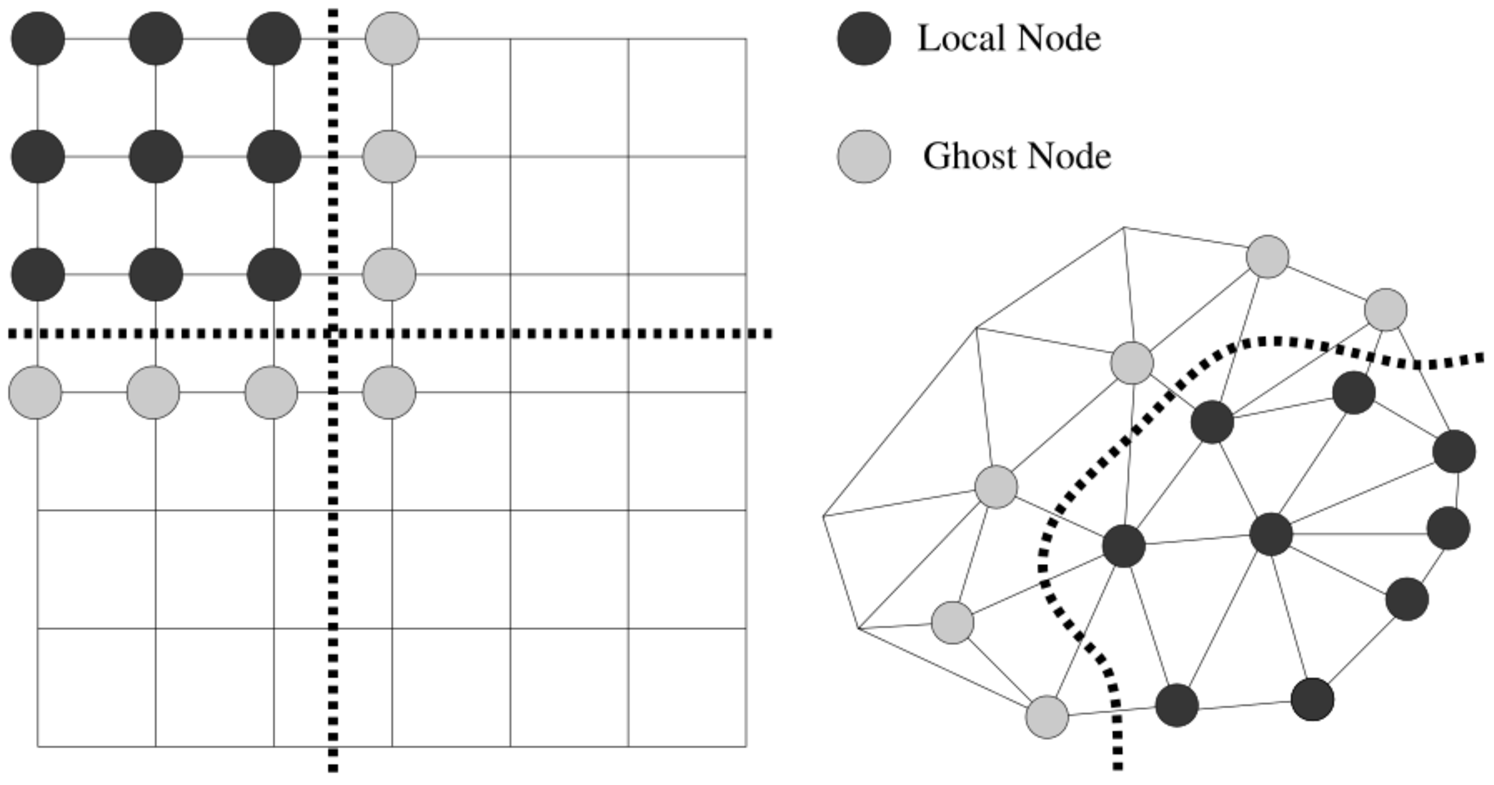
\includegraphics[width=\textwidth]{petscghostvalues}
\caption{\PETSc's parallel decomposition of structured and unstructured grids, showing owned (``local'') and accessible (``ghost'') nodes for one process.}
\label{fig:petscghostvalues}
\end{figure}

To wrap up our coverage of creating distributed grids, the standard \PETSc view of what \pDM s ``look like'' is in Figure \ref{fig:petscghostvalues}.  On the left is a version of what we have done in the code in Figure \ref{code:dmdacreatetwod}, namely create a structured grid \pDM.  The one shown in Figure \ref{fig:petscghostvalues} has \texttt{DMDA\_STENCIL\_BOX} stencil type, unlike ours.  On the right is an unstructured grid, of the type created in Chapter 3 for the finite element method.  In both cases the Figure shows the nodes owned by a given process (red ``local'' nodes) and those other nodes that are accessible by the local process (blue ``ghost'' nodes).  We will see such local/ghost node types in all examples in this book, and address their role again in future examples.


\section{Finite difference method: assemble the linear system}

Recall we were trying to approximate PDE problem \eqref{poissonsquare} and \eqref{poissonsquarebcs}!  Having built a structured grid we can now return to the FD method.

By a well-known Taylor's theorem argument \citep{MortonMayers}, for any function $F(x)$ which is sufficiently smooth, we have
\begin{equation}
   F''(x) = \frac{F(x+h) - 2 F(x) + F(x-h)}{h^2} + O(h^2)  \label{secondderivativeFD}
\end{equation}
as $h$ goes to zero.  This formula, applied to partial derivatives, will give an approximation of the Laplacian in equation\eqref{poissonsquare}.

Let $U_{i,j}$ be the gridded approximation to the value $u(x_i,y_j)$ of the exact solution $u(x,y)$ at a grid point,\sidenote{This is an important sentence!  We \emph{compute} values $U_{i,j}$ from the finite difference equations.  We generally \emph{don't know} the values $u(x_i,y_j)$.  Of course we want the former to be close to the latter.} and also denote $f_{i,j} = f(x_i,y_j)$.  From \eqref{secondderivativeFD} we have this FD approximation to equation \eqref{poissonsquare}:
\begin{equation}
- \frac{U_{i+1,j} - 2 U_{i,j} + U_{i-1,j}}{h_x^2} - \frac{U_{i,j+1} - 2 U_{i,j} + U_{i,j-1}}{h_y^2} = f_{i,j}. \label{poissonsquareFDearly}
\end{equation}
Equation \eqref{poissonsquareFDearly} applies for all of the interior points where $1 \le i \le M-2$ and $1 \le j \le N-2$.  The boundary conditions \eqref{poissonsquarebcs} become
\begin{equation}
U_{0,j} = 0, \quad U_{M-1,j} = 0, \quad U_{i,0} = 0, \quad U_{i,N-1} = 0, \label{poissonsquareFDbcs}
\end{equation}
for all $i,j$.

At a grid location $(x_i,y_j)$, equation \eqref{poissonsquareFDearly} relates the unknown $U_{i,j}$ to its four cardinal neighbors $U_{i+1,j}$, $U_{i-1,j}$, $U_{i,j+1}$, and $U_{i,j-1}$.  This pattern is a \emph{stencil}, in particular a ``star'' stencil, as shown in Figure \ref{fig:unitsquaregridstencil}.  A ``box'' stencil would additionally involve all the diagonal neighbors.  In 2D, a star stencil relates five unknowns, while a box stencil relates nine unknowns.

\begin{marginfigure}
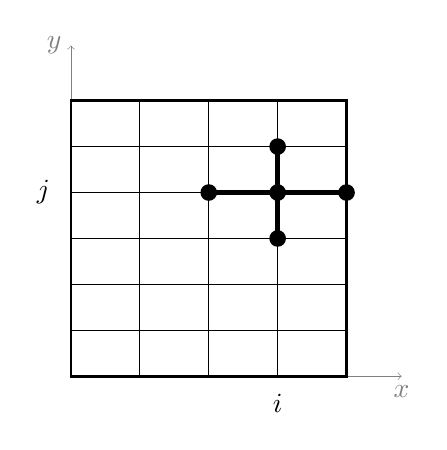
\begin{tikzpicture}[scale=3.5]
  \draw[->,gray,very thin] (0.0,0.0) -- (1.2,0.0) node[below] {$x$};
  \draw[->,gray,very thin] (0.0,0.0) -- (0.0,1.2) node[left] {$y$};
  \draw[line width=1.0pt] (0.0,0.0) -- (0.0,1.0) -- (1.0,1.0) -- (1.0,0.0) -- cycle;
  \node at (0.75,-0.1) {$i$};
  \node at (-0.1,0.666667) {$j$};
  \filldraw (0.50,0.666667) circle (0.8pt);
  \filldraw (0.75,0.666667) circle (0.8pt);
  \filldraw (1.00,0.666667) circle (0.8pt);
  \filldraw (0.75,0.5) circle (0.8pt);
  \filldraw (0.75,0.833333) circle (0.8pt);
  \draw[line width=2.0pt] (0.50,0.666667) -- (1.00,0.666667);
  \draw[line width=2.0pt] (0.75,0.5)  -- (0.75,0.833333);
  \draw[xstep=0.25,ystep=0.166667,black,thin] (0.0,0.0) grid (1.0,1.0);
\end{tikzpicture}
\caption{This ``star'' stencil simply illustrates the adjacency pattern in FD scheme \eqref{poissonsquareFDearly}.}
\label{fig:unitsquaregridstencil}
\end{marginfigure}

Equations \eqref{poissonsquareFDearly} and \eqref{poissonsquareFDbcs} form a linear system of $K=MN$ equations.  Note that if we choose to treat all values $U_{i,j}$ on the grid, whether on the boundary or in the interior, as unknowns then we have $K$ unknowns.  This is a linear
\begin{equation}
A \bu = \bb, \label{poissonlinearsystem}
\end{equation}
where $A$ is a $K\times K$ matrix and $\bu,\bb$ are $K\times 1$ column vectors.

But to shown this linear system in traditional form we must globally-order the unknowns.  Such an ordering is implemented inside a \PETSc \pDMDA, but a feature of \PETSc is that it is hidden and can often be ignored.  We are explicit about the ordering here for the purpose of displaying the system in matrix-vector form, but the code we actually write only uses the grid-wise coordinates $(i,j)$.  The ability to assemble \pMat s and \pVec s with $(i,j)$-type indexing is one reason \pDMDA codes can be quite short.

The ordering used in serial in a 2D \pDMDA is shown by example in Figure \ref{fig:unitsquaregridordering}.  On an $M$ by $N$ grid one could write the ordering as
\begin{equation}
    U_k = U_{i,j} \quad \text{ where } \quad k = j\,M + i \label{orderingfd}
\end{equation}
for $i=0,1,\dots,M-1$ and $j=0,1,\dots,N-1$, so $k=0,1,\dots,MN-1$.  As already noted, we will let \PETSc do such index transformations internally inside the \pDMDA implementation, but now we can show the linear system in a small-grid case.

\begin{marginfigure}
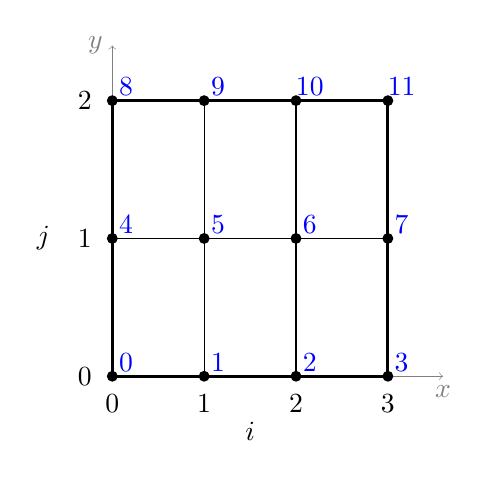
\begin{tikzpicture}[scale=3.5]
  \draw[->,gray,very thin] (0.0,0.0) -- (1.2,0.0) node[below] {$x$};
  \draw[->,gray,very thin] (0.0,0.0) -- (0.0,1.2) node[left] {$y$};
  \draw[line width=1.0pt] (0.0,0.0) -- (0.0,1.0) -- (1.0,1.0) -- (1.0,0.0) -- cycle;
  \pgfmathsetmacro\third{1.0/3.0}
  \pgfmathsetmacro\half{1.0/2.0}
  \node at (0.0,-0.1) {$0$};
  \node at (\third,-0.1) {$1$};
  \node at (\half,-0.2) {$i$};
  \node at (2*\third,-0.1) {$2$};
  \node at (1.0,-0.1) {$3$};
  \node at (-0.1,0.0) {$0$};
  \node at (-0.1,0.5) {$1$};
  \node at (-0.25,0.5) {$j$};
  \node at (-0.1,1.0) {$2$};
  \draw[xstep=\third,ystep=\half,black,thin] (0.0,0.0) grid (1.0,1.0);
  \pgfmathsetmacro\dd{0.05}
  \foreach \y in {0,1,2}
    \foreach \x in {0,1,2,3} {
      \pgfmathsetmacro\k{4*\y+\x}
      \draw[color=blue] (\x*\third+\dd,\y*\half+\dd) node{\pgfmathprintnumber[fixed]{\k}};
      \filldraw (\x * \third,\y * \half) circle (0.5pt);
    }
\end{tikzpicture}
\caption{Ordering of unknowns \eqref{orderingfd} on a $M=4$ and $N=3$ grid.  Index $k = j\,M + i$ is shown in {\color{blue} blue}.}
\label{fig:unitsquaregridordering}
\end{marginfigure}

\medskip\noindent\hrulefill
\begin{example} In the $M=4$ and $N=3$ case shown in Figure \ref{fig:unitsquaregridordering} we have grid spacing $h_x=1/3$ and $h_y=1/2$.  Equations \eqref{poissonsquareFDearly} and \eqref{poissonsquareFDbcs} are an invertible system of $K=12$ equations.  Only the $k=5$ and $k=6$ equations are not boundary conditions \eqref{poissonsquareFDbcs}.  The linear system is
\setcounter{MaxMatrixCols}{20}
\begin{equation*}
\begin{bmatrix}
1 &  &  &  &  &  &  &  &  &  &  &  \\
  & 1&  &  &  &  &  &  &  &  &  &  \\
  &  & 1&  &  &  &  &  &  &  &  &  \\
  &  &  & 1&  &  &  &  &  &  &  &  \\
  &  &  &  & 1&  &  &  &  &  &  &  \\
  & c&  &  & b& a& b&  &  & c&  &  \\
  &  & c&  &  & b& a& b&  &  & c&  \\
  &  &  &  &  &  &  & 1&  &  &  &  \\
  &  &  &  &  &  &  &  & 1&  &  &  \\
  &  &  &  &  &  &  &  &  & 1&  &  \\
  &  &  &  &  &  &  &  &  &  & 1&  \\
  &  &  &  &  &  &  &  &  &  &  & 1
\end{bmatrix}
\begin{bmatrix}
U_{0,0} \\
U_{1,0} \\
U_{2,0} \\
U_{3,0} \\
U_{0,1} \\
U_{1,1} \\
U_{2,1} \\
U_{3,1} \\
U_{0,2} \\
U_{1,2} \\
U_{2,2} \\
U_{3,2}
\end{bmatrix}
=
\begin{bmatrix}
0 \\
0 \\
0 \\
0 \\
0 \\
f_{1,1} \\
f_{2,1} \\
0 \\
0 \\
0 \\
0 \\
0
\end{bmatrix}
\end{equation*}
where $a = 2/h_x^2 + 2/h_y^2 = 26$, $b = - 1/h_x^2 = -9$ and $c = - 1/h_y^2 = -4$.

Note that the matrix $A$ is not symmetric.  Furthermore it is not well-scaled for such a small example.  For instance, its 2-norm condition number \citep{TrefethenBau} is $\cond(A) = \|A\|_2 \|A^{-1}\|_2 = 43.16$.
\end{example}
\noindent\hrulefill

Before assembling the system by writing \PETSc code, there are two nontrivial observations about it.  These observations lead to an equivalent linear system that is easier to solve.

First, the equations \eqref{poissonsquareFDearly} have very different ``scaling'' from those in \eqref{poissonsquareFDbcs} and this means that the rows of $A$ have very different scaling also.  For example, if $M=N=1001$, so that $h_x=h_y=0.001$, then the coefficient of $U_{i,j}$ in \eqref{poissonsquareFDearly} is $4/(.001)^2 = 4 \times 10^6$, while the coefficients along the boundary, from equations \eqref{poissonsquareFDbcs}, are equal to 1.

To make the equations better scaled, which is also the scaling that arises naturally in the finite element method (see Chapter 3), we multiply equation \eqref{poissonsquareFDearly} by the grid cell area $h_x h_y$ to get
\begin{align}
&\left(2 \frac{h_y}{h_x} + 2 \frac{h_x}{h_y}\right) U_{i,j} - \frac{h_y}{h_x}\left(U_{i+1,j} + U_{i-1,j}\right)  - \frac{h_x}{h_y}\left(U_{i,j+1} + U_{i,j-1}\right) \label{poissonsquareFD} \\
&\qquad = h_x h_y f_{i,j}. \notag
\end{align}
Using \eqref{poissonsquareFD}, in cases where the cell aspect ratio $\max\{h_y/h_x,h_x/h_y\}$ is not too large, all the equations in the system including the boundary conditions will have coefficients of comparable size.  If $h_x=h_y$ then the diagonal entries are equal to $4$ and the off-diagonal entries are $-1$; this is the well-known stencil shown in Figure \ref{fig:equalstarstencil}.

\begin{marginfigure}
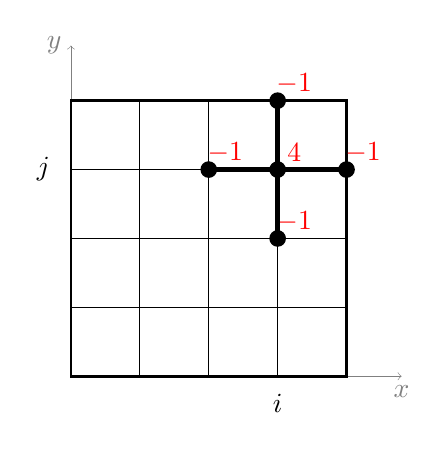
\begin{tikzpicture}[scale=3.5]
  \draw[->,gray,very thin] (0.0,0.0) -- (1.2,0.0) node[below] {$x$};
  \draw[->,gray,very thin] (0.0,0.0) -- (0.0,1.2) node[left] {$y$};
  \draw[line width=1.0pt] (0.0,0.0) -- (0.0,1.0) -- (1.0,1.0) -- (1.0,0.0) -- cycle;
  \node at (0.75,-0.1) {$i$};
  \node at (-0.1,0.75) {$j$};
  \filldraw (0.50,0.75) circle (0.8pt);
  \filldraw (0.75,0.75) circle (0.8pt);
  \filldraw (1.00,0.75) circle (0.8pt);
  \filldraw (0.75,0.5) circle (0.8pt);
  \filldraw (0.75,1.0) circle (0.8pt);
  \pgfmathsetmacro\dd{0.06}
  \draw[color=red] (0.75+\dd,0.75+\dd) node{$4$};
  \draw[color=red] (0.5+\dd,0.75+\dd)  node{$-1$};
  \draw[color=red] (0.75+\dd,0.5+\dd)  node{$-1$};
  \draw[color=red] (1.0+\dd,0.75+\dd)  node{$-1$};
  \draw[color=red] (0.75+\dd,1.0+\dd)  node{$-1$};
  \draw[line width=2.0pt] (0.50,0.75) -- (1.00,0.75);
  \draw[line width=2.0pt] (0.75,0.5)  -- (0.75,1.00);
  \draw[xstep=0.25,ystep=0.25,black,thin] (0.0,0.0) grid (1.0,1.0);
\end{tikzpicture}
\caption{For a grid with $h_x=h_y$, the coefficients on the left side of \eqref{poissonsquareFD}, shown here in {\color{red} red}, are the well-known ``$4$'' and ``$-1$'' for the stencil of the Laplacian.}
\label{fig:equalstarstencil}
\end{marginfigure}

Our second observation is that our FD equations can be re-interpreted to give a \emph{symmetric} matrix $A$.  This opens up a larger range of linear algebra methods for solving the system efficiently.  For example, in the $i=1$ case of \eqref{poissonsquareFD}, i.e.~at a grid point adjacent to the left-hand boundary of the square, the boundary location value $U_{0,j}$ appears in the equation.  The matrix in the linear system will be symmetric if we systematically ``move'' such values to the right-hand side as known.  That is, we force off-diagonal entries to be zero in columns corresponding to known boundary values, in addition to the existing off-diagonal zeros in the boundary-value rows.

With these two modifications we can redo the previous $M=4$ and $N=3$ example.

\medskip\noindent\hrulefill
\begin{example} For the same $M=4$ and $N=3$ case shown in Figure \ref{fig:unitsquaregridordering}, equations \eqref{poissonsquareFDbcs} and \eqref{poissonsquareFD} become
\begin{equation*}
\begin{bmatrix}
1 &  &  &  &  &  &  &  &  &  &  &  \\
  & 1&  &  &  &  &  &  &  &  &  &  \\
  &  & 1&  &  &  &  &  &  &  &  &  \\
  &  &  & 1&  &  &  &  &  &  &  &  \\
  &  &  &  & 1&  &  &  &  &  &  &  \\
  &  &  &  &  & \alpha& \beta&  &  &  &  &  \\
  &  &  &  &  & \beta& \alpha&  &  &  &  &  \\
  &  &  &  &  &  &  & 1&  &  &  &  \\
  &  &  &  &  &  &  &  & 1&  &  &  \\
  &  &  &  &  &  &  &  &  & 1&  &  \\
  &  &  &  &  &  &  &  &  &  & 1&  \\
  &  &  &  &  &  &  &  &  &  &  & 1
\end{bmatrix}
\begin{bmatrix}
U_{0,0} \\
U_{1,0} \\
U_{2,0} \\
U_{3,0} \\
U_{0,1} \\
U_{1,1} \\
U_{2,1} \\
U_{3,1} \\
U_{0,2} \\
U_{1,2} \\
U_{2,2} \\
U_{3,2}
\end{bmatrix}
=
\begin{bmatrix}
0 \\
0 \\
0 \\
0 \\
0 \\
(1/6) f_{1,1} \\
(1/6) f_{2,1} \\
0 \\
0 \\
0 \\
0 \\
0
\end{bmatrix}
\end{equation*}
where $\alpha = 2 (h_y/h_x) + 2 (h_x/h_y) = 13/3$ and $\beta = - h_y/h_x = - 3/2$.  The matrix is both symmetric and better-scaled, with $\cond(A)=5.83$.
\end{example}
\noindent\hrulefill

We now show the core code, in Figure \ref{code:structuredlaplacian}, that assembles ``$A$'' in our linear system \eqref{poissonlinearsystem}.  For clarity and code reuse we have isolated method \texttt{formdirichletlaplacian()} in a separate file.  We will use it both in the Poisson problem (\texttt{c2poisson.c}) and the time-dependent heat equation (\texttt{c2heat.c}) codes below.

\cinput{structuredlaplacian.c}{Fill matrix entries using \texttt{MatSetValuesStencil}.}{//CREATEMATRIX}{//ENDCREATEMATRIX}{code:structuredlaplacian}

The first action of \texttt{formdirichletlaplacian()} is to get a variable \texttt{info} of type  from the \pDM object \texttt{da}.  \texttt{DMDALocalInfo} is a C structure type which stores both global grid size and the size of the locally-owned grid.  This \texttt{struct} has the global grid size in members \texttt{info.mx,info.my} so we can compute grid spacings \texttt{hx,hy}.  The local process owns a \texttt{info.xm} by \texttt{info.ym} rectangular subgrid, with a range of indices
   $$\text{\texttt{info.xs}} \le i \le \text{\texttt{info.xs}} +\text{\texttt{info.xm}}-1$$
and
   $$\text{\texttt{info.ys}} \le j \le \text{\texttt{info.ys}} +\text{\texttt{info.ym}}-1$$
as shown in Figure \ref{fig:localpartofgrid}.  For example, in Figure \ref{fig:unitsquaregridparallel} the rank $0$ and $2$ processes have \text{\texttt{info.xs}}$=0$ and \text{\texttt{info.xm}}$=3$ while the rank $1$ and $3$ processes have \text{\texttt{info.xs}}$=3$ and \text{\texttt{info.xm}}$=2$.  (The $y$ ranges are similar.)  Such index ranges are then reflected in the \texttt{for} loops which re-appear every time we do operations on a structured 2D grid:
\begin{Verbatim}[fontsize=\small]
  for (j=info.ys; j<info.ys+info.ym; j++) {
    for (i=info.xs; i<info.xs+info.xm; i++) {
      DO SOMETHING AT OR NEAR GRID POINT (i,j)
    }
  }
\end{Verbatim}

\begin{marginfigure}
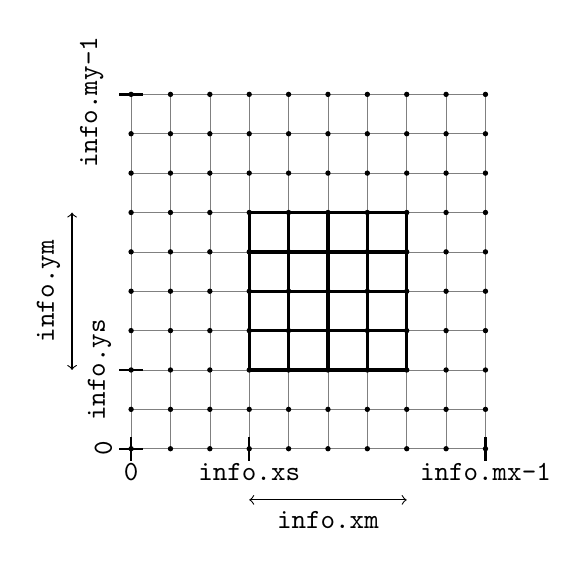
\begin{tikzpicture}[scale=5]
  % global grid, local grid, nodes
  \draw[xstep=0.1,ystep=0.1,gray,very thin] (0.0,0.0) grid (0.9,0.9);
  \draw[xstep=0.1,ystep=0.1,black,very thick] (0.3,0.2) grid (0.7,0.6);
  \foreach \y in {0,...,9}
    \foreach \x in {0,...,9} {
      \filldraw (\x * 0.1,\y * 0.1) circle (0.15pt);
    }
  % ticks on x-axis at 0, xs, mx
  \draw[black,thick] (0,-0.03)   -- (0,+0.03);
  \draw[black,thick] (0.3,-0.03) -- (0.3,+0.03);
  \draw[black,thick] (0.9,-0.03) -- (0.9,+0.03);
  \node at (0,-0.06) {\texttt{0}};
  \node at (0.3,-0.06) {\texttt{info.xs}};
  \node at (0.9,-0.06) {\texttt{info.mx-1}};
  % ticks on y-axis at 0, ys, my
  \draw[black,thick] (-0.03,0)   -- (+0.03,0);
  \draw[black,thick] (-0.03,0.2) -- (+0.03,0.2);
  \draw[black,thick] (-0.03,0.9) -- (+0.03,0.9);
  \node[rotate around={90:(0,0)}] at (-0.07,0) {\texttt{0}};
  \node[rotate around={90:(-0.2,0.2)}] at (-0.08,0.12) {\texttt{info.ys}};
  \node[rotate around={90:(0.0,0.9)}] at (-0.28,0.7) {\texttt{info.my-1}};
  % xm, ym along sides of local patch
  \draw[<->,] (0.3,-0.13) -- (0.7,-0.13);
  \node at (0.5,-0.18) {\texttt{info.xm}};
  \draw[<->,] (-0.15,0.2) -- (-0.15,0.6);
  \node[rotate around={90:(0.3-0.3,0.4)}] at (-0.29,0.32) {\texttt{info.ym}};
\end{tikzpicture}
\caption{How the \texttt{DMDALocalInfo info} struct describes the indices for a local process' part of a 2D grid, and the global grid size, using six integers.}
\label{fig:localpartofgrid}
\end{marginfigure}

The \pMat object $A$ which is assembled by \texttt{formdirichletlaplacian()} in Figure \ref{code:structuredlaplacian} has ranges of rows owned by each process.  This is the standard parallel layout of \pMat objects in \PETSc.  But this fact is another one that we don't need to know, on a \pDMDA-managed structured grid.  Instead we work with our locally-owned part of the grid using the $(i,j)$ description of a point and its stencil neighbors.  Such local indices can be used when inserting entries into a dynamical data structure for matrix assembly, namely the non-yet-assembled \pMat.

Thus in Figure \ref{code:structuredlaplacian} we see one command \texttt{MatSetValuesStencil()} for each locally-owned grid point.  For a generic interior point this command inserts five coefficients into the matrix.  The key data structure is of type \texttt{MatStencil}, an apparently-trivial struct
\begin{Verbatim}[fontsize=\small]
typedef struct {
  PetscInt k,j,i,c;
} MatStencil;
\end{Verbatim}
In our 2D case, with a single degree of freedom at each node,\sidenote{The Poisson equation \eqref{poissonsquare} is a scalar PDE so the unknown at each grid point is the scalar $U_{i,j}$.  A system of equations like Navier-Stokes would have \texttt{dof}$>1$ when we call \texttt{DMDACreateXd()}.} we only use the \texttt{i} and \texttt{j} members of \texttt{MatStencil}.  From \eqref{poissonsquareFD}, the actual matrix entries are $a_{i,i} = 2\left(h_y/h_x + h_x/h_y\right)$ on the diagonal or $a_{i,j} = -h_y/h_x$ or $a_{i,j} = -h_x/h_y$ for off-diagonals.  As mentioned above, we only insert nonzero off-diagonals in the matrix if the column corresponds to a non-boundary location.  After completing all the \texttt{MatSetValuesStencil()} insertion commands we call 
\begin{Verbatim}[fontsize=\small]
  MatAssemblyBegin(A,MAT_FINAL_ASSEMBLY);
  MatAssemblyEnd(A,MAT_FINAL_ASSEMBLY);
\end{Verbatim}
just as we did in Chapter 1.


\section{Finite difference method: manufacture a problem}

At this point we can set up a particular Poisson problem and proceed to solve it.  So that we know the exact solution we choose it,\sidenote{This same problem appears in Chapter 4 of \citep{Briggsetal2000}.  We are not being original!}% page 64
taking care that it satisfies the boundary conditions:
\begin{equation}
u(x,y) = (x^2 - x^4) (y^4 - y^2). \label{exactsolution}
\end{equation}
Note that $u=0$ along $\partial \mathcal{S}$.  Then we just differentiate to get $f$ so that $-\grad^2 u=f$ and thus \eqref{exactsolution} solves \eqref{poissonsquare}:
\begin{equation}
f(x,y) = 2 (1 - 6 x^2) y^2 (1 - y^2) + 2 (1 - 6 y^2) x^2 (1 - x^2).\label{manufacturedf}
\end{equation}
Furthermore, noting that the truncation error term ``$O(h^2)$'' in equation \eqref{secondderivativeFD} has a coefficient which is proportional to the fourth derivative, our finite difference method will not be exact, which is the generic case.

\cinputpart{c2poisson.c}{This method assembles a \pVec for the right-hand side of equation \eqref{poissonsquareFD}, and one for the exact solution.  Only local grid coordinates $(i,j)$ are used.}{I}{//RHS}{//ENDRHS}{code:ctwopoissonrhs}

Since $u$ from \eqref{exactsolution} and $f$ from  \eqref{manufacturedf} are intimately-connected, we isolate the code which computes these two functions in a method called \texttt{formRHSandExact()}, shown in Figure \ref{code:ctwopoissonrhs}.  As explained above we compute all the entries of the \pVec objects using only local grid coordinates $(i,j)$.  \PETSc pointer ``tricks'' allow us to index the C arrays we get from \texttt{DMDAVecGetArray()}, which have type \texttt{double **} = \texttt{PetscReal **}, using these grid indices.  (Recall Figure \ref{fig:localpartofgrid}.)  When we are done with the computation part we must both restore the C arrays by calling \texttt{DMDAVecRestoreArray()}, and explicitly ask for the \pVec objects to be assembled by calling \texttt{VecAssemblyBegin/End()}.

Now we can get started on solving the whole problem using \PETSc.  Figure \ref{code:ctwopoissoncreate} shows how \texttt{c2poisson.c} creates the various parallel objects needed to solve the Poisson problem, especially one \pDM, one \pMat, and three \pVec s.  Note that a \pDM object possesses, or can compute, the matrix and vector sizes from the grid dimensions, so we call \texttt{DMCreateMatrix()} and \texttt{DMCreateGlobalVector()}, respectively, to create the \pMat and the \pVec s.  We also indicate the matrix-assembly part of the code to \PETSc's performance-logging API; more on that later.  Then we call the methods \texttt{formdirichletlaplacian()} and \texttt{formRHSandExact()}, which have already been shown.

\cinputpart{c2poisson.c}{Set up \pDMDA \texttt{da} and \pMat \texttt{A} objects, and assemble the latter by calling \texttt{formlaplacian()}.}{II}{//CREATE}{//ENDCREATE}{code:ctwopoissoncreate}

\cinputpart{c2poisson.c}{Solve using \pKSP, and report on solution.}{III}{//SOLVE}{//ENDSOLVE}{code:ctwopoissonsolve}


\section{Does our method work?: demonstrate convergence}


\section{Runtime control of linear solver}

FIXME: basic Krylov theory

\section{Time-dependent heat equation}

FIXME: we WON'T do explicit, but it would look like ...

FIXME: use TS for backward-euler
